\begin{section}{Kombinatorische Definitionen}
  Um über Graphen und deren Färbbarkeit sinnvoll reden zu können, müssen zuerst einige gebräuchliche Definitionen gemacht werden. 
 
  \begin{definition}{Graph, Knoten, Kante}
    \-\ 
    \begin{itemize}
    \item Ein \textit{Graph} $G$ ist ein Paar $G=(V,E)$, wobei $V$ eine endliche Menge ist, deren Elemente \textit{Knoten} genannt werden, und $E$ eine endliche Menge bestehend aus Kanten sind.
    \item Eine \textit{Kante} $e \in E$ ist eine zweielementige Teilmenge von $V$, wobei $E$ die Menge aller dieser Teilmengen ist, also $E \subseteq \{\{u,v\}|u,v \in V, u \neq v\}$.
    \item Die Menge der Knoten eines Graphen $G$ wird auch mit $V(G)$ bezeichnet, die Menge der Kanten mit $E(G)$.
    \end{itemize}
  \end{definition}
  
  Oft werden wir auch die Bausteine einer Landkarte $\mathcal{L}$ als Knoten- und Kantenmenge verwenden. Die Ecken von $\mathcal{L}$ werden zu den Knoten des Graphen, die Jordanbögen von $\mathcal{L}$ zu den Kanten des Graphen. Im weiteren betrachten wir vorwiegend endliche Graphen, außer es wird explizit anders angegeben. Auch schließt diese Definition Schleifen explizit aus. Schleifen sind Kanten, bei denen $u=v$ gilt. Schleifen müssen bei Färbbarkeitsüberlegungen ausgeschlossen werden, denn könnte ein Knoten zu sich selbst benachbart sein, wäre es nicht möglich, für benachbarte Knoten stets unterschiedliche Farben zu wählen.\\
  Um nun Bedingungen an die Färbbarkeit von Graphen stellen zu können, muss noch definiert werden, wie dessen Knoten zusammenhängen.
 
  \begin{definition}{Inzidenz, Adjazenz, Knotengrad, vollständiger Graph}
    Sei $G=(V,E)$ ein Graph. Dann sind die folgenden Bezeichnungen gebräuchlich:
    \begin{itemize}
    \item Ein Knoten $v \in V$ heißt \textit{inzident} zu einer Kante $e \in E$, wenn mindestens eines der Elemente von $e$ der Knoten $v$ ist, also $v \in e$. 
    \item Zwei verschiedene Knoten $u,v$ heißen \textit{adjazent}, wenn sie zur gleichen Kante inzident sind, d.h. $\{u,v\}\in E$
    \item Für einen Knoten $v$ ist der \textit{Grad} von $v$ definiert als die Anzahl der Kanten, die zu $v$ adjazent sind. Es gilt $d_G(v) = \sharp\{\{v,b\} \in E | b\in V\}$.
    \item Ein Graph $G$ heißt \textit{vollständig}, wenn gilt: $E = \binom{V}{2} = \{\{u,v\}|u,v \in V, u \neq v\}$.
   \end{itemize}
  \end{definition}
    
  Für eine interessante Struktur benachbarter Knoten gibt es eine gebräuchliche Bezeichnung, auf die wir später zurückgreifen werden.
  
  \begin{definition}{Pfad, einfacher Pfad, disjunkte Pfade, Kreis, Ring}
  Sei $G=(V,E)$ ein Graph.
   \begin{itemize}
    \item Eine Folge $(v_1,\cdots,v_r)$ von mindestens drei Knoten heißt \textit{Pfad}, wenn die auftretenden Knoten paarweise verschieden, aber je zwei aufeinanderfolgenden benachbart sind. Dann ist $r$ die Länge der Kette und die Verbindungskanten heißen Glieder.
    \item Ein Pfad heißt \textit{einfach}, wenn zwei seiner Knoten nur dann benachbart sind, wenn sie im Pfad aufeinanderfolgenden. Oder genauer: Für die Indizes $j_1, j_2 \in \{1,\cdots,r\}$ mit $|j_1 - j_2| > 1$ sind die Knoten des Pfades $v_{j_1}$ und $v_{j_2}$ nicht benachbart.
    \item Zwei Pfade heißen \textit{disjunkt}, wenn sie keine Knoten, die nicht erstes oder letztes Element der jeweiligen Folge sind, gemeinsam haben. 
    \item Ein Pfad heißt \textit{Kreis}, wenn $v_1$ und $v_r$ ebenfalls benachbart sind.
    \item Ein \textit{Ring} ist ein Kreis, der zusätzlich einfach ist.
   \end{itemize}
  \end{definition}
  
  Ringe werden im Allgemeinen als wesentlicher Beitrag von Birkhoff auf dem Weg zur Lösung des 4-Farben-Problems angesehen, zuerst erwähnt in \cite{AmJMath35}.

  Einiges Handwerkszeug ist noch nötig, um Strukturen prägnant und kurz beschreiben zu können.
  
  \begin{definition}{Teilgraph $G\setminus X$, $G\setminus Y$}
   Sei $G=(V,E)$ ein Graph, $X \subseteq V$ eine Teilmenge der Knoten und $Y \subseteq E$ eine Teilmenge der Kanten. Weiter sei $F$ die Menge der Kanten $f$ aus $V$ mit $f \cap X \neq \emptyset$. Der Graph $G\setminus X = (V\setminus X,E\setminus F)$ unterscheidet sich von $G$ derart, dass alle Knoten der Menge $X$ und alle zu diesen Knoten adjazenten Kanten gelöscht werden. Ebenso ist $G\setminus Y = (V,E\setminus Y)$ der Graph, bei dem alle Kanten aus $Y$ entfernt wurden.
  \end{definition}
  
  \begin{definition}{Kontraktion}
   Durch \textit{Kontraktion} erhält man aus einem Graphen einen Teilgraphen, indem man zwei adjazente Knoten $v_1$ und $v_2$ zusammenfasst. Man sagt, man kontrahiert $v_2$ auf $v_1$, wenn man $v_2$ aus dem ursprünglichen Graphen entfernt und alle Kanten, zu denen $v_2$ inzident ist, zu $v_1$ führt. Dabei werden jene Kanten zu Knoten entfernt, wenn diese bereits zu $v_1$ adjazent waren.
  \end{definition}

  Betrachtet man diesen Vorgang aus topologischer Sicht, entspricht eine Kontraktion einer Vereinigung zweier benachbarter Länder durch Aufheben ihrer gemeinsamen Grenze.
  
  Da das Problem der 4-Färbbarkeit von Graphen von der Geographie motiviert ist, betrachten wir als Raum für unsere Knoten nur den $\mathbb{R}^2$, also die Ebene.
  
  \begin{definition}{Planarität}
   Ein Graph heißt \textit{planar}, wenn seine Kanten so in der Ebene durch Jordanbögen darstellbar sind, dass sich diese höchstens in ihren Endpunkten schneiden.
  \end{definition}
  
  Damit man sich planare Graphen noch leichter vorstellen kann, fügen wir hier noch folgendes Resultat ein.
  
  \begin{satzl}{Wagner und Fáry}{WagFar}
   Jeder Graph kann durch einen Homöomorphismus der Ebene auf sich in einen Streckengraphen überführt werden.
  \end{satzl}
  
  Dieser Satz liefert uns, dass es sich bei diesen Jordanbögen tatsächlich stets um gerade Verbindungsstrecken handeln kann. Für den Beweis dieses Resultats verweisen wir auf \cite[Seite 113]{fritsch}, da er nur der Darstellung von Graphen nutzt und wenig zum eigentlichen Beweis beiträgt. 
  
  Planarität von Graphen wirkt auf den ersten Blick wie ein rein topologischer Begriff, jedoch gelang es Kuratowski, eine rein kombinatorische Charakterisierung von Planarität zu liefern.
  
  \begin{satz}{Kuratowski}
   Ein Graph ist genau dann planar, wenn er sich durch (möglicherweise) mehrfache Kontraktion nicht in einen der beiden Graphen $K_{3,3}$ oder $K_5$ überführen lässt.
  \end{satz}
  
  Auch dieser Beweis findet sich in der gängigen Literatur und wird daher an dieser Stelle nicht geführt. Jedoch wollen wir die beiden genannten Graphen kurz aufzeigen. Auf der linken Seite ist die übliche Darstellung der $K_5$ zu finden, auf der rechten Seite die des $K_{3,3}$.
  
  \[ 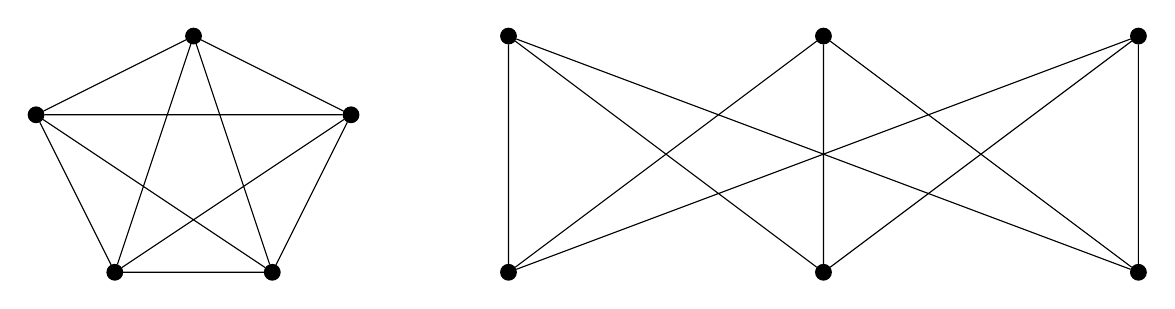
\begin{tikzpicture}[every node/.style={draw,inner sep=2pt,fill=black}]
      \path[shape=circle]
	(2,3) node(a1){} (6,0) node(x1){} (10,0) node(x2){} (14,0) node(x3){} 
	(0,2) node(b1){} (4,2) node(b2){}
	(1,0) node(c1){} (3,0) node(c2){}  (6,3) node(y1){} (10,3) node(y2){} (14,3) node(y3){};
	\filldraw (a1) -- (b1) -- (c1) -- (c2) -- (b2) -- (a1) -- (c1) -- (b2) -- (b1) -- (c2) -- (a1);
	\filldraw (x1) -- (y1) -- (x2) -- (y2) -- (x3) -- (y3) -- (x1) -- (y2);
	\filldraw (x2) -- (y3);
	\filldraw (y1) -- (x3);
\end{tikzpicture} \]

  Wir werden die Jordanbögen der Darstellung eines Graphen ebenfalls als \textit{Kanten} bezeichnen. In der Ebene ist es leicht, die durch diese Kanten getrennten Flächen zu betrachten. Das führt uns zur folgenden Definitionen.
  
  \begin{definition}{Facette, Außenfacette}
   Sei $G$ ein in der Ebene $\mathbb{R}^2$ gezeichneter Graph. Sei $J_G$ die Menge der Jordanbögen dieser Darstellung.
   \begin{itemize}
   \item Eine \textit{Facette} ist eine Zusammenhangskomponente von $\mathbb{R}^2 \setminus J_G$. Die Endpunkte der Kanten, die die Facette umfassen heißen ebenfalls inzident zu dieser Facette. 
   \item Der unbeschränkte Rest der Ebene, der von keiner Menge von Kanten vollständig umschlossen ist, wird \textit{Außenfacette} genannt.
   \end{itemize}
  \end{definition}
  
  Um die Außenfacette vollständig charakterisieren zu können, bedarf es eigentlich des Jordanschen Kurvensatzes. Dieser kann bei \cite[Seite 53]{fritsch} nachgelesen werden.
  
  Weiter gibt es einige gebräuchliche Namenskonventionen für Knoten, um deren Lange im Graphen genauer zu charakterisieren.
  
  \begin{definition}{Außenknoten, Innenknoten}
   Sei $G$ ein in der Ebene gezeichneter Graph.
   \begin{itemize}
    \item Jeder Knoten, der inzident zur Außenfacette von $G$ ist, wird \textit{Außenknoten} genannt.
    \item Jeder Knoten von $G$, der kein Außenknoten ist, ist automatisch ein \textit{Innenknoten}.
   \end{itemize}

  \end{definition}

  Für unsere Betrachtungen ist eine besondere Form von Facetten interessant. 
  
  \begin{definition}{Dreieck, Triangulation, Beinahe-Triangulation}
   Sei $G$ ein in der Ebene gezeichneter Graph.
   \begin{itemize}
   \item Eine Facette ist genau dann ein \textit{Dreieck}, wenn genau drei Knoten zu ihr inzident sind. Ein Ring ist genau dann ein Dreieck, wenn er aus drei Knoten besteht.
   \item Ein planarer Graph ist eine \textit{Triangulation}, wenn er schleifenfrei und jede seiner Facetten ein Dreieck ist. 
   \item Eine \textit{Beinahe-Triangulation} ist ein nichtleerer, schleifenfreier, planarer Graph $G$, bei dem jede beschränkte Facette ein Dreieck ist. 
   \end{itemize}
  \end{definition}
  
  Zeichnet man die Kanten eines planaren Graphen als gerade Linien, so entspricht diese Definition genau dem, was man sich unter einem Dreieck vorstellt. Das dies auch tatsächlich möglich ist, werden wir am Ende des Kapitels kurz diskutieren. Der Unterschied zwischen einer Triangulation und einer Beinahe-Triangulation liegt lediglich in der Form der Außenfacette des Graphen. 
 
  \begin{definition}{Färbung, Farben, Gültigkeit}
   Sei $G=(V,E)$ ein Graph.
   \begin{itemize}
   \item Eine \textit{Färbung} ist eine lineare Abbildung $f: V \leftarrow \mathbb{N}$, die jedem Knoten eines Graphen eine natürliche Zahl zuordnet. 
   \item Die Elemente von $C  =f(V)$ nennt man \textit{Farben}. 
   \item Eine Färbung heißt \textit{gültig}, wenn sie keinem Paar adjazenter Knoten $u,v \in V$ die gleiche Farbe zuordnet, also $c(u) \neq c(v)$ für $\{u,v\}\in E$. 
   \end{itemize}
  \end{definition}
  
  \begin{definition}{$k$-Färbbarkeit}
   Ein Graph $G$ heißt \textit{$k$-färbbar}, wenn für eine gültige Färbung von $G$ mit höchstens $k$ Farben gibt.
  \end{definition}
  
  Aus dieser Definition ergibt sich auch direkt, dass jeder $k$-färbbare Graph auch $(k+1)$-färbbar ist. Nun haben wir alle nötigen Definitionen zusammen, um unsere ersten Resultate zu zeigen. Das erste dient vorallem der vereinfachten Veranschaulichung, das zweite werden wir später noch benötigen.
  
  \begin{satzl}{Vollständiger Graph mit fünf Knoten}{voll5}
   Es existiert kein vollständiger planarer Graph mit fünf Knoten.
  \end{satzl}
  \begin{proof}
    Es seien $v_1,\cdots,v_5$ fünf Ecken in der Ebene. Für jedes Paar $i,j \in \{1,2,3,4,5\}$ mit $i < j$ sei eine Kante $k_{i,j}$ zwischen $v_i$ und $v_j$ gegeben. Dieser Graph hat $10$ Kanten, von denen insgesamt $7$ entweder $v_1$ oder $v_5$ oder beide als Endpunkt haben. Wir zeigen nun, dass sich mindestens eine der $3$ übrigen Kanten eine der anderen Kanten überkreuzen muss.\\
    Durch Zusammensetzen erhält man drei Pfade $P_i = k_{1,i} \cup k_{i,5}$ für $i = 2,3,4$, die die Knoten $v_1$ und $v_5$ verbinden, die sich aber weder untereinander noch mit $k_{1,5}$ schneiden. O.B.d.A. sei $P_3$ der Pfad derart, dass von den beiden anderen einer in der Facette $F$ und der andere außerhalb der Facette $F$ begrenzt von $k_{1,5} \cup P_3$ liegt. Damit muss die Kante $k_{2,4}$ zwischen $v_2$ und $v_4$ mindestens einen inneren Punkt $y$ mit dem Rand von $F$ gemeinsam haben, also mit einer der Kanten $k_{1,5},k_{1,3},k_{3,5}$. Da $k_{2,4}$ keine der drei beteiligten Ecken trifft, muss $y$ ein innerer Punkt einer dieser Kanten sein.
  \end{proof}
  
  Dieser Beweis ist ebenfalls in \cite[Satz 4.1.2]{fritsch} zu finden, allerdings in einer topologischen Variante mittels Jordanbögen. 
  
 \begin{satzl}{Weiske}{weiske}
  Es gibt keine Landkarte $\mathcal{L}$ mit fünf paarweise benachbarten Ländern.
 \end{satzl}
 \begin{proof}
  Angenommen, es gäbe eine solche Landkarte. Betrachte dazu die zu $\mathcal{L}$ duale Landkarte. Diese ist ein Graph mit 5 Ecken, die paarweise verbunden sind. Einen solchen Graphen kann es aber nach \nameref{voll5} nicht geben. Widerspruch.
 \end{proof}
\end{section}